\subsection{Tools > Distances > Cloud/Mesh dist.}
\label{subsection:cloud2meshDist}

\begin{figure}[!htb]
\begin{center}
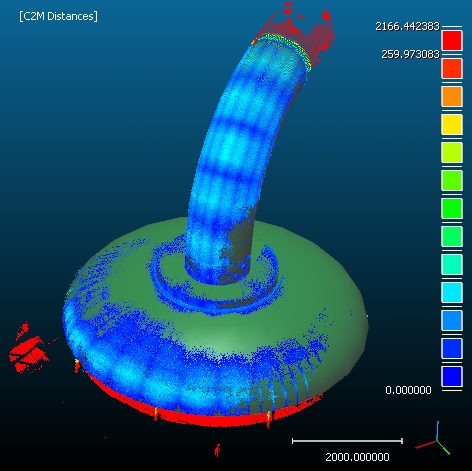
\includegraphics[width=0.4\textwidth]{Partie3_Fonctions/cloud2MeshDistExample.jpg}
\caption{\label{fig:cloud2MeshDistExample}Exemple de r�sultat de calcul de distances entre un nuage et un maillage}
\end{center}
\end{figure}


Cette fonction permet de calculer les distances\index{distances} (approximatives ou exactes) entre un nuage de points et un maillage.
\\
\par
Cette fonction est largement �quivalente au calcul de distances entre nuages (section~\ref{subsection:cloud2cloudDist}) mis � part
quelques d�tails :
\begin{itemize}
\item si un seule des deux entit�s s�lectionn�es est un maillage, le choix des r�les (section~\ref{subsection:chooseRole}) n'est
pas n�cessaire (le maillage est forc�ment l'entit� de r�f�rence).
\item si les deux entit�s s�lectionn�es sont des maillages, les sommets de l'entit� \emph{compar�e} seront utilis�s en guise de
\emph{nuage}. Il peut �tre int�ressant d'utiliser la fonction d'�chantillonnage\index{echantillonner@�chantillonner!des points sur un maillage} de points sur un maillage (Cf.
section~\ref{subsection:samplePoints}) pr�alablement, pour avoir une meilleure vision des diff�rences entre maillages
(si cela est le r�sultat escompt�).
\item cette fonction rajoute un champ scalaire \emph{C2M Distances} au nuage de r�f�rence (nuage compar�).
\item le choix d'une mod�lisation locale (\emph{Local model}) n'est pas possible puisque l'entit� de r�f�rence est ici un maillage.
\end{itemize}
